O desenvolvimento do projeto NitrusLeaf foi estruturado em etapas organizadas de forma sequencial e iterativa, com base em princípios de desenvolvimento ágil, visando flexibilidade e adaptação ao longo do processo. O método adotado busca garantir a integração eficiente entre as etapas de análise, implementação e validação dos resultados, assegurando a qualidade e a aplicabilidade da solução desenvolvida.

\medskip
\noindent\textbf{Escopo atual (MVP).} Aplicação web funcional (front-end em React/Next.js e back-end em Node.js) com cadastro e armazenamento de dados em MySQL; planejamento do pipeline de visão computacional e coleta/organização inicial de dados.

\medskip
\noindent\textbf{Escopo alvo (versão completa).} Integração do classificador baseado em CNN em produção, implantação em nuvem, ponto de captura padronizado em campo (IoT) e avaliação de eficiência por análise de algoritmos (latência, throughput e uso de memória).
\medskip

A Figura \ref{fig:fluxograma} apresenta o fluxograma geral do processo metodológico, descrevendo a sequência lógica das atividades realizadas, desde a captura das imagens até o registro final dos diagnósticos no sistema.

\begin{figure}[H]
    \centering
    \caption{Fluxograma do processo de classificação das folhas de mexerica}
    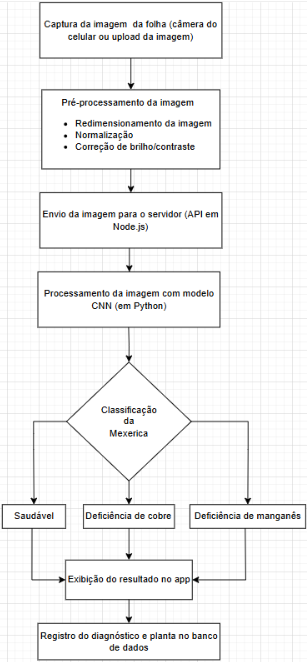
\includegraphics[width=0.6\linewidth]{Illustrations/fluxograma.png}
    \label{fig:fluxograma}
    \SourceOrNote{Fonte: autoria própria (2025)}
\end{figure}

A seguir, descrevem-se detalhadamente as etapas que compõem o processo metodológico representado no fluxograma:

\begin{enumerate}
\item \textbf{Coleta de Requisitos e Planejamento do Sistema}

Nesta etapa inicial, foram levantados os requisitos funcionais e não funcionais do sistema, definindo-se as principais funcionalidades e fluxos de interação. Para o planejamento da interface e prototipagem, utilizou-se o Figma, devido à sua facilidade de colaboração e à capacidade de criar protótipos interativos de baixa e alta fidelidade. Essa fase também incluiu a elaboração de diagramas UML para a representação da estrutura do sistema e análise SWOT para identificar forças, fraquezas, oportunidades e ameaças, garantindo uma visão ampla do projeto.

\item \textbf{Captura e Pré-processamento das Imagens}

O processo tem início com a captura de imagens de folhas de mexerica por meio da câmera do celular ou upload de imagens previamente armazenadas. As imagens passam por etapas de pré-processamento, incluindo redimensionamento, normalização e correção de brilho e contraste. Essas operações garantem a padronização dos dados visuais, fundamentais para o bom desempenho da CNN durante a classificação.

\item \textbf{Envio e Processamento das Imagens}

Após o pré-processamento, as imagens são enviadas para o servidor por meio de uma API desenvolvida em Node.js. No servidor, o modelo de IA implementado em Python realiza o processamento utilizando redes neurais convolucionais (CNNs) treinadas previamente com imagens rotuladas de folhas saudáveis e com deficiências de cobre e manganês. Essa etapa representa o núcleo analítico do sistema, onde ocorre a classificação automática das imagens.

\item \textbf{Classificação e Exibição dos Resultados}

O modelo realiza a classificação das folhas em três categorias: saudável, deficiência de cobre ou deficiência de manganês. O resultado é exibido no aplicativo em tempo real, fornecendo ao usuário um diagnóstico rápido e acessível. Essa abordagem visa permitir a identificação imediata de deficiências no campo, reduzindo o tempo entre o diagnóstico e a tomada de decisão pelo agricultor.

\item \textbf{Registro e Armazenamento dos Diagnósticos}

Os diagnósticos gerados são armazenados no banco de dados, associados ao registro da planta e ao talhão correspondente. Essa funcionalidade possibilita o acompanhamento histórico do estado nutricional das plantas, facilitando análises posteriores e o monitoramento contínuo das condições do cultivo.

\item \textbf{Treinamento e Avaliação do Modelo}

O treinamento do modelo de IA foi realizado a partir de um conjunto de imagens rotuladas, aplicando técnicas de \textit{data augmentation} para aumentar a diversidade visual do conjunto. Foram utilizadas métricas de desempenho como acurácia, precisão e F1-score para validar o modelo. A metodologia de avaliação segue princípios semelhantes aos empregados por \textcite{Tran2019}, que demonstraram a importância da validação cruzada e da comparação de arquiteturas para garantir resultados consistentes e confiáveis.

\item \textbf{Ferramentas Utilizadas}

Para a implementação do sistema, foram empregadas diferentes ferramentas tecnológicas. O front-end foi desenvolvido com React e Next.js, oferecendo desempenho otimizado e boa organização estrutural. O back-end foi construído em Node.js, responsável pela integração com o banco de dados e a comunicação com o modelo de IA. O armazenamento de dados foi realizado com MySQL, escolhido pela robustez e ampla compatibilidade. O módulo de visão computacional foi desenvolvido em Python, pela facilidade de integração com bibliotecas voltadas à IA, como TensorFlow e Keras.


\end{enumerate}
%---------------------------------------------------------
\subsection{Pesquisa de campo}
Durante a pesquisa de campo realizada com produtores de fazendas de \textit{Citrus reticulata} (mexerica), ambas localizadas no município de Pariquera-Açu, foram entrevistados os produtores identificados como \textbf{Entrevistado A} e \textbf{Entrevistado B}, os quais relataram experiências relevantes relacionadas ao manejo nutricional e fitossanitário em suas propriedades.

\medskip
O \textbf{Entrevistado A} relatou que, em sua fazenda, já ocorreram deficiências de manganês e 
cobre nas plantas de \textit{Citrus reticulata} (mexerica). A suspeita surgiu devido ao amarelamento das 
folhas e à clorose internerval. A correção dessas deficiências foi realizada por meio da adubação 
com fertilizantes enriquecidos com os nutrientes necessários. O entrevistado afirmou conseguir 
distinguir alguns casos de deficiência de manganês e cobre e relatou já ter tido contato com a 
doença \textit{Greening}, identificada por sintomas como amarelamento e presença do 
\textit{Psilídeo}; 
nesses casos, houve perda total dos frutos. Em sua fazenda, a falta de nutrientes é frequente, 
sendo o diagnóstico realizado por indicadores como amarelamento das folhas, frutos pequenos e 
produção reduzida. Mais da metade dos casos diagnosticados refere-se a deficiências nutricionais
gerais. O entrevistado também destacou que um dos principais problemas enfrentados é o controle 
de pragas, e que, quando há algum problema na saúde das plantas, busca auxílio de técnico ou 
agrônomo. Além disso, realiza a verificação da saúde das plantas uma vez por mês. Ele e sua 
equipe contam com o auxílio de aplicativos e o apoio de especialistas para a verificação e 
controle das plantações.

O \textbf{Entrevistado B} relatou ter enfrentado problemas de deficiência de manganês e cobre 
em suas plantas, cuja identificação ocorreu por meio do diagnóstico realizado por um 
engenheiro agrônomo, que indicou as medidas corretivas. Em algumas ocasiões, esse profissional 
também realiza análise foliar. O entrevistado afirma conseguir distinguir as deficiências 
nutricionais da doença \textit{Greening} por meio da observação de sintomas, e relata já ter 
tido \textit{Greening} em sua fazenda. O diagnóstico baseia-se na experiência dos funcionários 
e na observação do estado da árvore e dos frutos, porém é tardio, pois as alterações nas 
folhas ocorrem somente em plantas já afetadas. Existem casos em que a planta continua 
produzindo frutos saudáveis mesmo estando doente; nesses casos, o pé não é cortado, apenas 
tratado, para evitar a disseminação da doença para outras plantas. Houve perda parcial da 
plantação devido ao \textit{Greening}, mas havia possibilidade de recuperação. 
Também são frequentes o amarelamento, a perda e a diminuição dos frutos na fazenda. 
O entrevistado afirma que a maioria dos casos de deficiência nutricional está relacionada 
à falta de manganês. Os principais problemas enfrentados no cotidiano da plantação são a 
falta de conhecimento da maioria dos colaboradores para identificar problemas de saúde nas 
plantas de \textit{Citrus reticulata} (mexerica), o que se deve, em parte, ao predomínio do 
cultivo de banana na região, reduzindo o conhecimento específico sobre a cultura cítrica. 
Quando ocorre algum problema na plantação, é chamado um técnico para avaliar e corrigir 
eventuais problemas, como ácaros nos frutos, e as deficiências nutricionais acabam ficando 
em segundo plano. O entrevistado realiza monitoramento da saúde das plantas em média uma vez 
por semana, geralmente por meio da observação dos funcionários durante o trabalho no pomar. 
Regularmente, não são utilizadas tecnologias para medir a saúde das plantas, mas, pontualmente,
foram empregadas adesivos amarelos para atrair insetos transmissores do \textit{Psilídeo}, 
drones para testar a aplicação de caldas e marcação com fita plástica para monitorar plantas 
suspeitas de \textit{Greening}.

\medskip

Diante das observações realizadas durante a pesquisa de campo, evidencia-se a importância deste 
estudo para a melhoria das práticas de manejo nutricional e fitossanitário nas plantações de 
\textit{Citrus reticulata} (mexerica). Verificou-se que o diagnóstico das deficiências 
nutricionais, especialmente de manganês e cobre, ainda ocorre de forma tardia e, em muitos 
casos, é confundido com sintomas da doença \textit{Greening}, resultando em perdas significativas
na produção e no descarte de plantas potencialmente produtivas.

\medskip

O presente projeto propõe o desenvolvimento de um método de diagnóstico precoce das 
deficiências nutricionais por meio da análise foliar automatizada, reduzindo a necessidade 
de acompanhamento técnico constante e facilitando o monitoramento direto pelos produtores.

\medskip


